\ProvidesPackage{preamble}
\usepackage[utf8]{inputenc}
\usepackage[T1]{fontenc,url}
\usepackage{babel,textcomp}
\usepackage{graphicx}
\usepackage{pdfpages}
\usepackage{fancyhdr}
\usepackage{afterpage}
\usepackage{amsmath}
\usepackage{amssymb}
\usepackage{caption}
\usepackage{mathtools}
\usepackage{listings}
\usepackage{color}
\usepackage[margin=1.2in]{geometry}

%\usepackage[hidelinks]{hyperref} % make links black
\usepackage{hyperref}
%\hypersetup{
  %colorlinks=false,
  %colorlinks=true,
  % citecolor=black,
  % filecolor=black,
  % linkcolor=red,
  % urlcolor=blue,
  % linktoc=all,
  % linktocpage,
%}

\pagestyle{fancy}
\fancyhead{}
\fancyfoot{}
\renewcommand{\headrulewidth}{0.0pt}
\renewcommand{\footrulewidth}{0.0pt}
\fancyhead[R]{\thepage}
\fancyhead[L]{\emph{}}

\renewcommand{\vec}[1]{\mathbf{#1}}    % vektorer i bf fremfor pil
\let\oldhat\hat
\renewcommand{\hat}[1]{\oldhat{\mathbf{#1}}} % enhetsvektorer i bf med hatt

\definecolor{keywords}{RGB}{50,50,250}
\definecolor{comments}{RGB}{190,70,20} % Orange
\definecolor{red}{RGB}{160,0,0}
\definecolor{green}{RGB}{0,150,0}
\definecolor{grey}{RGB}{225,225,225}

\lstdefinestyle{terminal}
{
  frame=single,
  basicstyle=\ttfamily,%\small,
}

\lstdefinestyle{fortran}
{
  frame=shadowbox,
  rulesepcolor=\color{black},
  language=Fortran,
  basicstyle=\ttfamily,%\small,
  keywordstyle=\bf\color{keywords},
  morekeywords={as,range,len,float},
  commentstyle=\color{comments},
  stringstyle=\color{red},
  showstringspaces={false}
}

\lstdefinestyle{python}
{
  %frame=shadowbox,
  rulesepcolor=\color{black},
  language=Python,
  basicstyle=\ttfamily,%\small,
  keywordstyle=\bf\color{keywords},
  morekeywords={as,range,len,float},
  commentstyle=\color{comments},
  stringstyle=\color{red},
  showstringspaces={false}
}
  % numbers=left,                     # Numbered lines
  % numbersep=5pt,                    # Dist from num to code
  % numberstyle=\small,%\color{mygray},
  % identifierstyle=\color{green}%,
  % backgroundcolor=\color{},
  % emph={MyClass,__init__},          % Custom highlighting
  % emphstyle=\ttb\color{deepred}}    % Custom highlighting style

% Custom commands
\newcommand{\pder}[2]{\frac{\partial #1}{\partial #2}}
\newcommand{\ppder}[2]{\frac{\partial^2 #1}{\partial^2 #2^2}}
\newcommand{\half}{\frac{1}{2}}
\newcommand{\intO}{\int_{\Omega}}
\newcommand{\intdO}{\int_{\partial\Omega}}
\newcommand{\intu}{\int^1_{-1}}
\newcommand{\ti}[1]{\tilde{#1}}
\newcommand{\md}{\;\mathrm{d}}
\newcommand{\ha}[1]{\text{\^{#1}}}

\title{
	{Thesis Title}\\
	{\large Institution Name}\\
}
\author{Author Name}
\date{Day Month Year}

\usepackage{amsmath,amsfonts,amssymb,amsthm,epsfig,epstopdf,titling,url,array}
\theoremstyle{definition}
\newtheorem{defn}{Definition}[section]
\newtheorem{conj}{Conjecture}[section]
\newtheorem{exmp}{Example}[section]
\usepackage{listings}
\usepackage{amsmath}
\title{Benchmark}
\author{Sebastian Gjertsen}
\begin{document}
\maketitle



\newpage

\section*{Problem Defintion}
\subsection*{Domain}
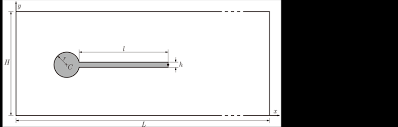
\includegraphics[scale=0.9]{geometry.png}
The computational domain resembles the classic cfd benchmark with an added bar, with dimensions: \\
The box: L = 2.5, H = 0.41 \\
The bar: l = 0.35, h = 0.02 \\s
The circle is positioned at (0.2, 0.2) making it 0.05 of center from bottom to top, this is done to induce oscillations to an otherwise laminar flow.\\
Boundary conditions:\\
The fluid velocity has a parabolic profile on the inlet that changes over time:\\
$$ u(0,y) = 1.5u_0 \frac{y(H-y)}{(\frac{H}{2})^2}  $$
$$ u(0,y,t) = u(0,y)\frac{1-cos(\frac{\pi}{2}t)}{2} \text{  for  } t<2.0$$
$$ u(0,y,t) = u(0,y) \text{  for  } t \leq 2.0 $$

We set no slip on the "floor" and "ceiling" so to speak.\\
On the fluid solid interface the boundary conditions are set to:
$$  \sigma_f n_f = \sigma_s n_s \hspace{4mm} on  \hspace{2mm}\Gamma^0 (interface)   $$
In our variational form we leave this out and so implying that they are equal.

\subsection*{CSM test}
Parameters
\begin{table}[h]
\centering
\caption{My caption}
\label{my-label}
\begin{tabular}{|l|l|l|l|}
\hline
Parameters & CSM1 & CSM2 & CSM3 \\ \hline
$\rho_f[10^3 \frac{kg}{m^3}]$ & 1 & 1 & 1 \\ \hline
$\nu_f [10^{-3} \frac{m^2}{s}]$ & 1 & 1 & 1 \\ \hline
$u_0$ & 0 & 0 & 0 \\ \hline
$\rho_s[10^3 \frac{kg}{m^3}]$ & 1 & 1 & 1 \\ \hline
$\nu_s$ & 0.4 & 0.4 & 0.4 \\ \hline
$\mu_s[10^6 \frac{m^2}{s}]$ & 0.5 & 2.0 & 0.5 \\ \hline
$g $ & 2 & 2 & 2 \\ \hline
\end{tabular}
\end{table}


\begin{figure}[ht] 
  \label{ fig7} 
  \begin{minipage}[b]{0.6\linewidth}
    \centering
    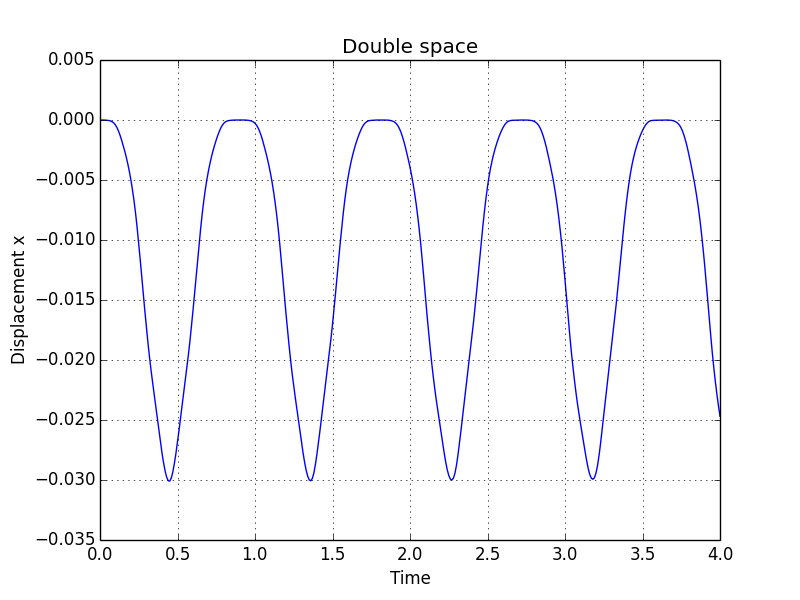
\includegraphics[width=1\linewidth]{med_diff_x.png} 
    \caption{diff x with diffusion term} 
    \vspace{4ex}
  \end{minipage}%%
  \begin{minipage}[b]{0.6\linewidth}
    \centering
    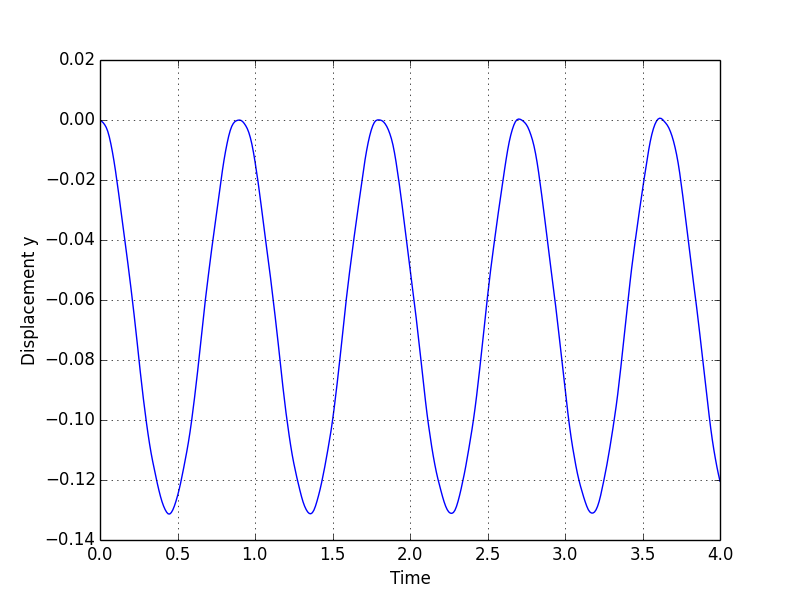
\includegraphics[width=1\linewidth]{med_diff_y.png} 
    \caption{diff y with diffusion term} 
    \vspace{4ex}
  \end{minipage} 
  \begin{minipage}[b]{0.6\linewidth}
    \centering
    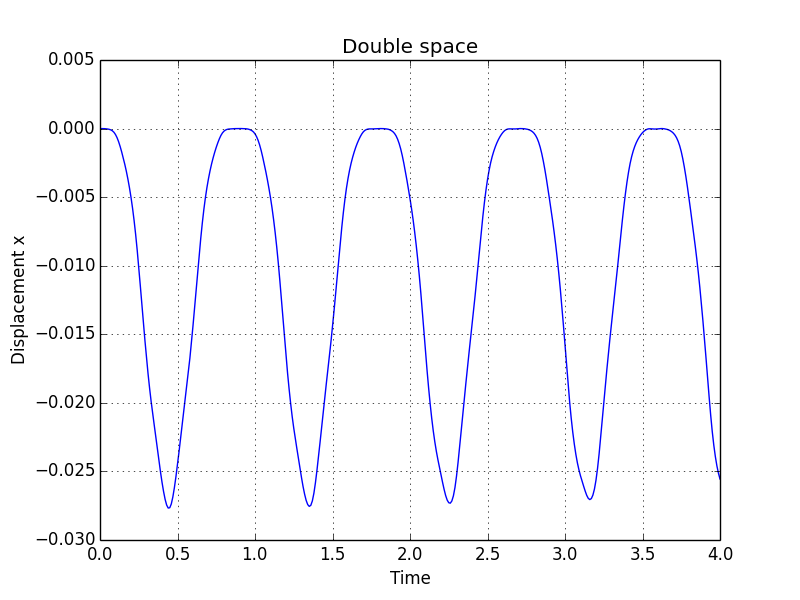
\includegraphics[width=1\linewidth]{uten_diff_x.png} 
    \caption{diff x without diffusion term} 
    \vspace{4ex}
  \end{minipage}%% 
  \begin{minipage}[b]{0.6\linewidth}
    \centering
    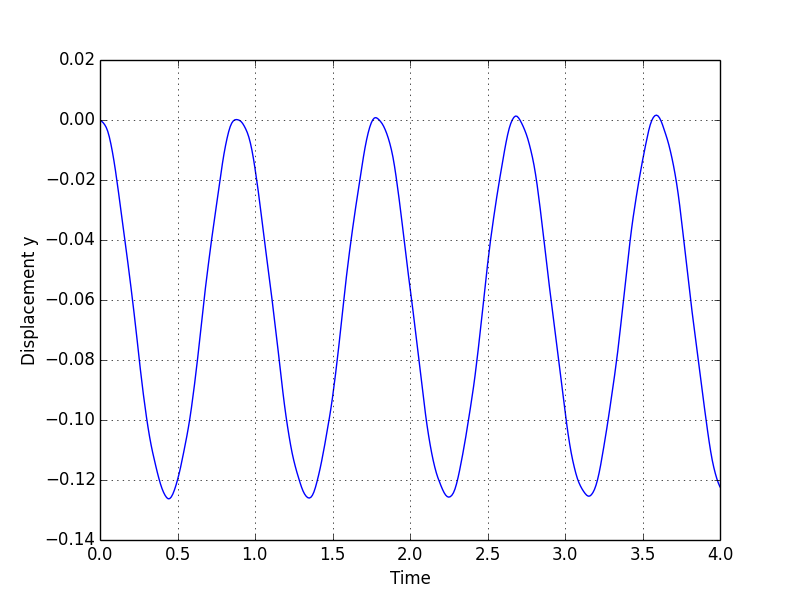
\includegraphics[width=1\linewidth]{uten_diff_y.png} 
    \caption{diff y without diffusion term} 
    \vspace{4ex}
  \end{minipage} 
\end{figure}



\newpage
\newpage 

\subsection*{FSI test}
\begin{table}[h]
\centering
\caption{My caption}
\label{my-label}
\begin{tabular}{|l|l|l|l|}
\hline
Parameters & FSI1 & FSI2 & FSI3 \\ \hline
$\rho_f[10^3 \frac{kg}{m^3}]$ & 1 & 1 & 1 \\ \hline
$\nu_f [10^{-3} \frac{m^2}{s}]$ & 1 & 1 & 1 \\ \hline
$u_0$ & 0.2 & 1 & 2 \\ \hline
Re = $\frac{U d}{\nu_f}$ & 20 & 100 & 200 \\ \hline
$\rho_s[10^3 \frac{kg}{m^3}]$ & 1 & 10 & 1 \\ \hline
$\nu_s$ & 0.4 & 0.4 & 0.4 \\ \hline
$\mu_s[10^6 \frac{m^2}{s}]$ & 0.5 & 0.5 & 2 \\ \hline
\end{tabular}
\end{table}
Results: 
\begin{table}[ht]
\centering
\caption{My caption}
\label{my-label}
\begin{tabular}{|l|l|l|l|l|l|l|}
\hline
Cells & Dofs & ux of A $[�10^{-3}]$ & uy of A $[�10^{-3}]$ & Drag & Lift & Spaces \\ \hline
2698 & 7095 & 0.0213214 & 1.01342 & 14.1679 & 0.942656 & P1-P1-P1 \\ \hline
2698 & 23563 & 0.02271 & 0.80288 & 14.1736 & 0.787891 & P2-P2-P1 \\ \hline
10792 & 92992 & 0.0227341 & 0.808792 & 14.1855 & 0.801044 & P2-P2-P1 \\ \hline
43168 & 369448 & 0.227352 & 0.812595 & 14.227 & 0.797242 & P2-P2-P1 \\ \hline
\textbf{ref} & \textbf{ref} & \textbf{0.0227} & \textbf{0.8209} & \textbf{14.295} & \textbf{0.7638} & \textbf{ref} \\ \hline
\end{tabular}
\end{table}


\bibliographystyle{plain}
@article{quaini2014extended,
  title={An extended ALE method for fluid-structure interaction problems with large structural displacements},
  author={Quaini S ?Canic, S Basting A and Glowinski, R},
  year={2014}
}
\bibliography{./Cite/cites}

\end{document}
